\section{Implementation Details}
With the terminology in place we are now ready to describe the implementation of our parallel algorithm. First, however, we will go into a bit of detail on why our initial approach to solving this problem was unfruitful, such that others might learn from our mistakes.

Recall that the overall goal for this implementation is to construct an $n$ by $m$ matrix $A$, $n$ being the number of lines for each scan and $m$ being the number of angles. Within $A$ the $(i, j)$'th entry should contain an array representing a sparse matrix. This array should represent the scan-grid where each pixel (each entry of the array) has the intersection length of the $i$'th line at the $j$'th angle increment with that pixel.

\subsection{Targeting a parallel machine}
When implementing a program that is meant to run in parallel, programmers are faced with the challenge that their go-to strategies might not be good fits for the parallel execution model that they are targeting. Unfamiliarity with the model leads to writing programs that have inefficient behavior on the machine, which was also the case at times during this project. Our initial approach was to parallelize across all three parameters, i.e. angles, lines and individual intersections. As mentioned each intersection point between the line and the grid must have integer $x$- or $y$-components. Knowing this, we created two arrays with increasing integer values corresponding to grid coordinates, one for $x$ and one for $y$. To avoid unnecessary calculations, we calculated the entry- and exit points of the line passing through the grid and set the size and values of the two arrays accordingly.  Mapping over the two arrays with the standard linear equation produced two sorted arrays of grid intersections, which could then be merge-sorted to produce a single sorted array of intersections. 

This method proved inefficient, even before starting to compute the actual lengths between the intersections. To ensure that programs have good performance on the GPU, \texttt{Futhark} enforces \emph{regular arrays}. This means that each array in a collection of arrays must all have the same length. Anecdotally this is because all kernels should use the same amount of memory for its execution. The two arrays that needed merging often had different lengths from one line to another, which in turn made the resulting arrays irregular lengths. Some attempts were made to pad with zeroes to reach a common length but ultimately we could not get the code to run on the GPU due to the irregular arrays. Futhermore, it is also said that on the GPU too much branching logic within a single kernel should be avoided, especially when the branching differs across kernels. The act of sorting involves a lot of branching so it became clear that another methodology, one better suited for the parallel execution model, was needed.

\subsection{A Working Solution}
As revealed to us in the discussion on the degree of parallelization in section \ref{sec:degOfPar} we should parallelize over each line, even across angle increments. This is done in Futhark using nested \texttt{map}s which means that for each line a sequential algorithm is run. The overall strategy, per line, is this: First compute the points where the line enters and exits the grid. Then the line can be traversed iteratively starting from the entry and ending at the exit point. As this traversal happens, a result array representing the grid can be updated with lengths.

\textbf{Initialization}\newline
First off, three things are computed: The center point of the grid, the slope of the line and its intersection with the y-axis (using equations \eqref{eq:slope} and \eqref{eq:y_intersection}). These are used to find the points of the line that lie on the perimeter of the grid. The one with the lowest x-component is by convention called the entry point and the other is the exit. This convention lets us always traverse the line in the increasing direction of the x-axis. From these two points two indices are computed, called \texttt{anchorX} and \texttt{anchorY} respectively. The meaning of these will be apparent in the coming section. Depending on whether the slope is negative or positive we should traverse the line with decreasing or increasing y-values respectively. This direction is also computed at this point.
\begin{figure}[H] 
  \centering
  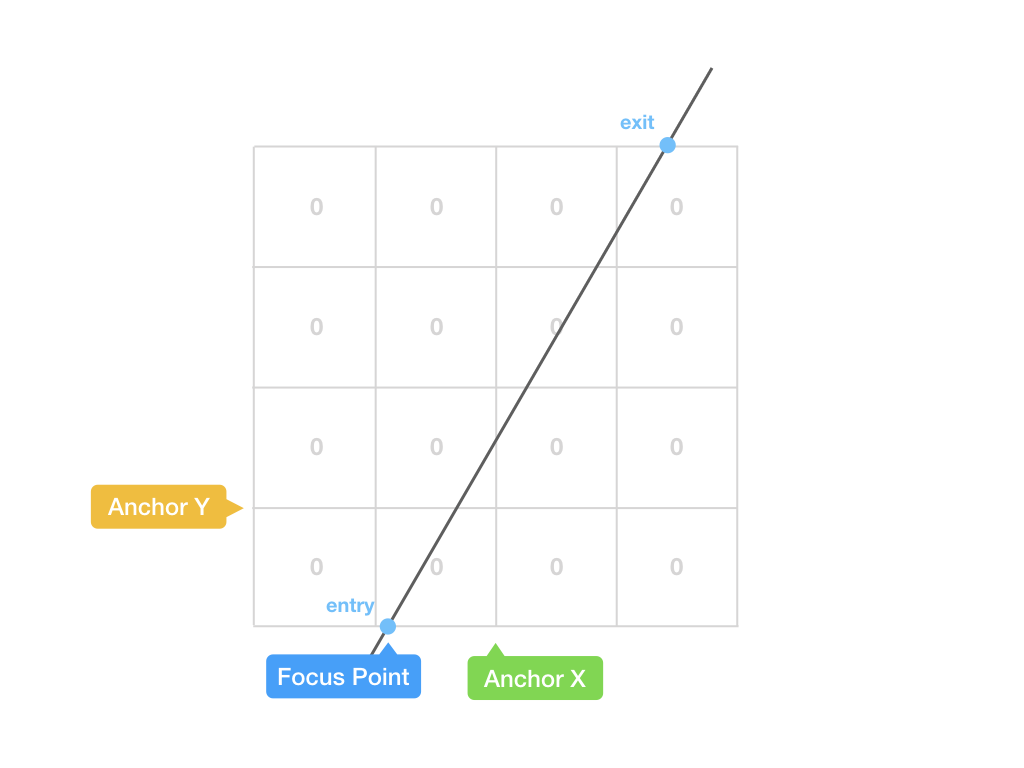
\includegraphics[width=0.8\textwidth]{figures/alg_init.png}
  \caption{Starting state of the algorithm}
  \label{fig:alg_init}
\end{figure}
Since Futhark is a functional language it does not support iterative code per say. It does provide some control structures that have a strong resemblance to common iterative code though. In our case we use a \texttt{loop} structure with a \texttt{while}-clause. The way it works is that one can update an object via an expression until a certain condition is met. This object is in our case a quadruple with the following contents:
\begin{enumerate}
  \item The result array \texttt{A} which is a flat representation of the grid. This is updated with a new length per iteration. To ensure regular arrays \texttt{A} is initialized with $2 \cdot q - 1$ entries that are all (-1, -1).
  \item\texttt{focusPoint} which is the point from which the algorithm decides what to do in the iterative step. Initially this is set to the entry point.
  \item\texttt{anchorX} which is used for control on the horizontal axis. It always contains the smallest x-value that is larger than the x-component of \texttt{focusPoint}. Put another way it contains the next index on the x-axis where the line intersects with the grid.
  \item\texttt{anchorY} which corresponds to \texttt{anchorX} only on the vertical axis.
\end{enumerate}
\textbf{The i'th step}
\begin{figure}[H] 
  \centering
  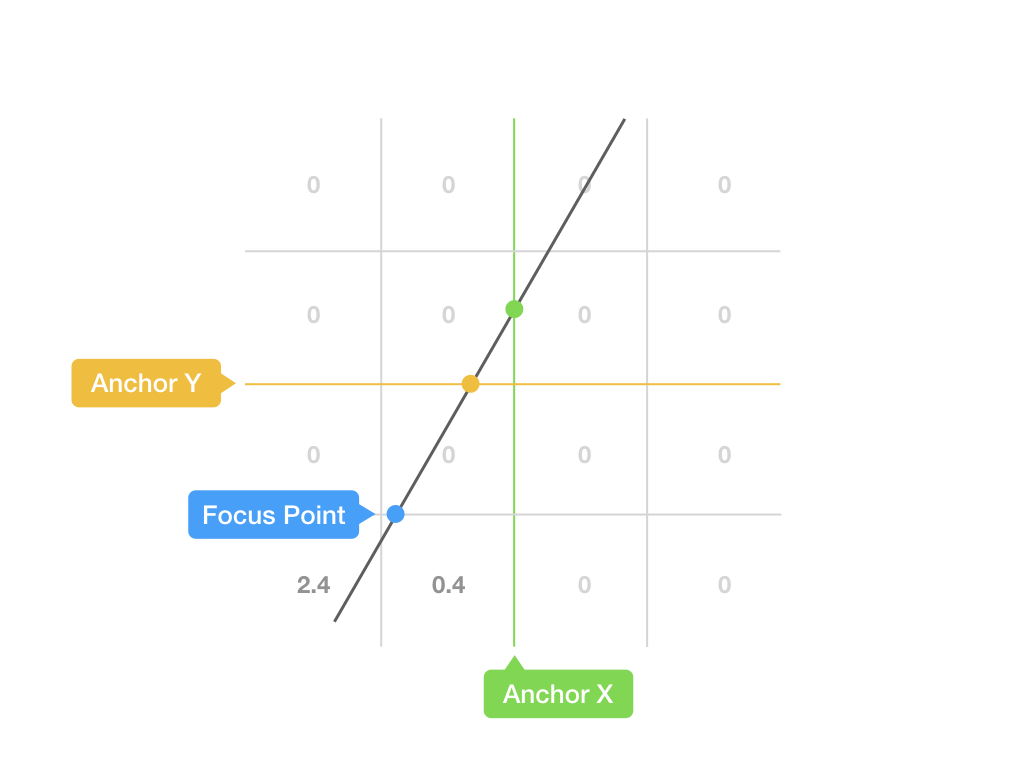
\includegraphics[width=0.8\textwidth]{figures/alg_step_before.png}
  \caption{The general state of the algorithm before taking the i'th step.}
  \label{fig:alg_step_before}
\end{figure}
Figure \ref{fig:alg_step_before}  illustrates the situation at the start of each iteration. If we trace along the line starting from \texttt{focusPoint} until we hit another grid-line then that intersection is bound to have either \texttt{anchorX} as its x-component or \texttt{anchorY} as its y-component. This means that to get the next intersection we can simply compute the points that lie on the line and has these anchors as a component. Let us call these \texttt{p\_anchorX} (the green dot in fig. \ref{fig:alg_step_before}) and \texttt{p\_anchorY} (the orange dot). Then, to decide which of these points should be the next \texttt{focusPoint}, we compute the distance to each point. The one that is closest to the current \texttt{focusPoint} is then chosen. The distance to this closest point is written into \texttt{A} at the index of the pixel that the line-segment lies within. Note that this index is computable from the components of \texttt{focusPoint}. Now we should update the anchors for the next iteration. If the closest point was \texttt{p\_anchorY} then \texttt{anchorY} must be either incremented or decremented depending on the y-direction (the one that was computed from the slope of the line). Due to the way we chose the entry and exit points we know that if \texttt{p\_anchorX} was chosen then we should simply increment \texttt{anchorX}. Figure \ref{fig:alg_step_after} reflects the resulting new state.
\begin{figure}[H]
  \centering
  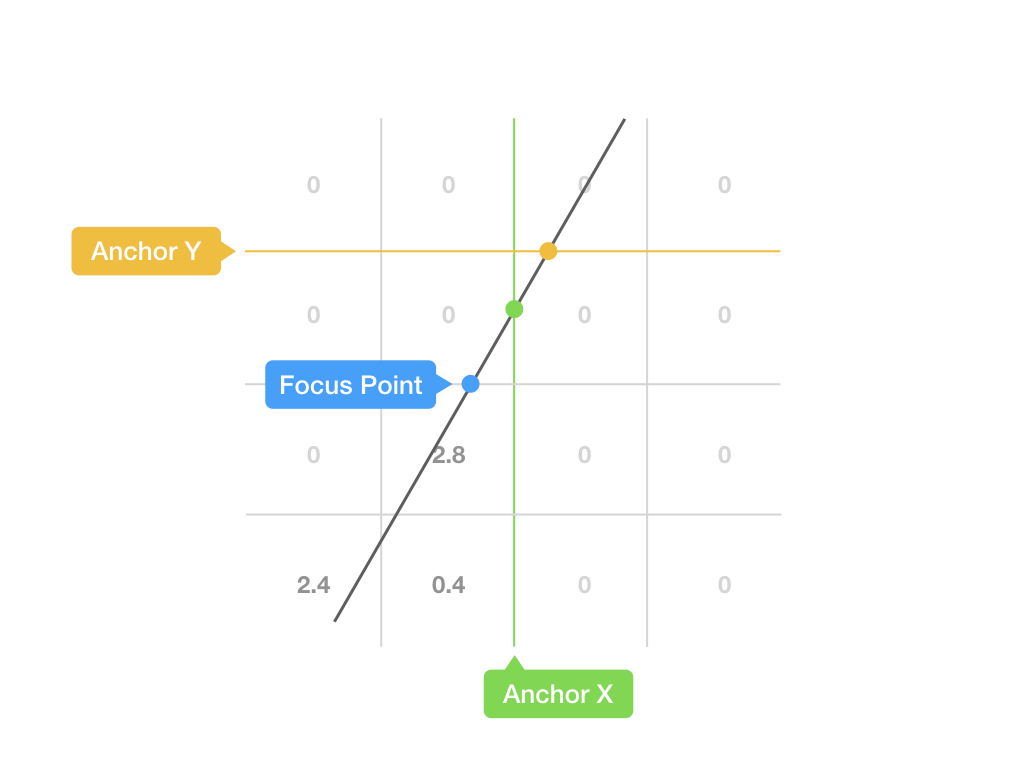
\includegraphics[width=0.9\textwidth]{figures/alg_step_after.png}
  \caption{The resulting state taking the i'th step.}
  \label{fig:alg_step_after}
\end{figure}
\newpage
\textbf{Termination}\\
Moving onto the termination step, our algorithm has a very simple exit condition on its loop-structure: When the \texttt{focusPoint} lies on the perimeter of the grid the loop should be exited. This situation is illustrated in figure \ref{fig:alg_step_term}. Do note that depending on the y-direction some edge-cases needs handling. This is because the entry point lies on the perimeter as well, so one should think that the algorithm never gets started. This caveat is taken care of in a small specialized function \texttt{isInGrid} that considers the y-direction when determining whether the point is on the perimeter. That is, if the y-direction is positive then a \texttt{focusPoint} with y-component equal to 0 does not stop the loop while a y-component equal to the grid-size does (and vice versa for negative y-directions). When the loop has terminated the computation is done and the algorithm returns the result \texttt{A}.
\begin{figure}[H] 
  \centering
  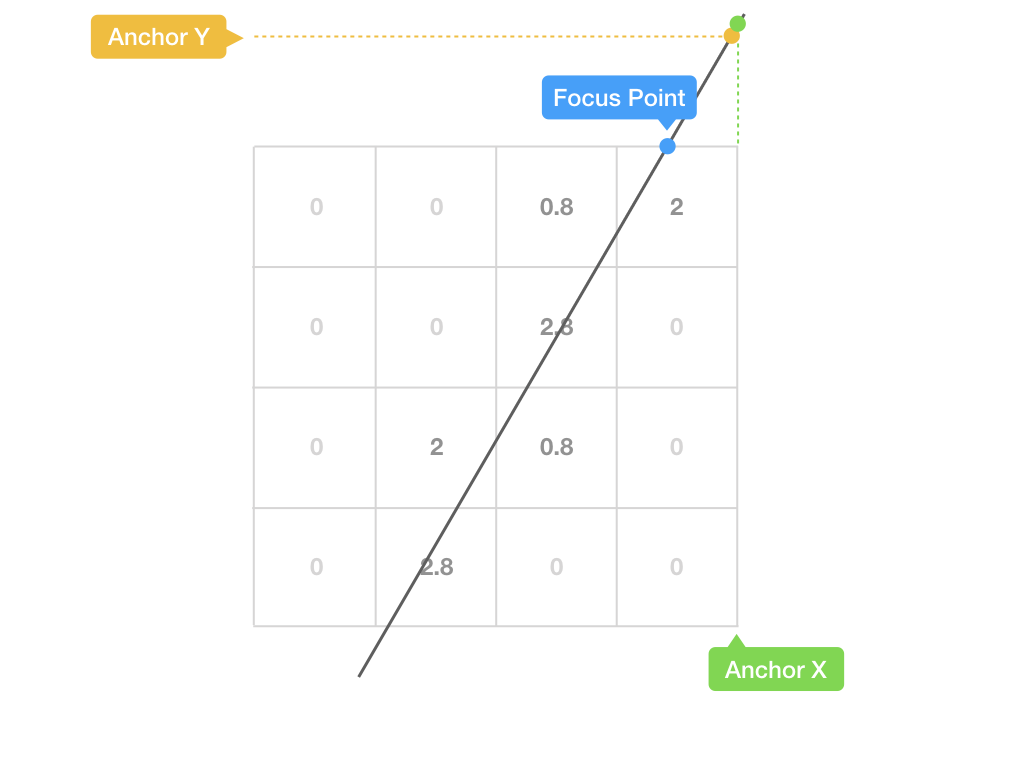
\includegraphics[width=0.9\textwidth]{figures/alg_term.png}
  \caption{The termination of the algorithm.}
  \label{fig:alg_step_term}
\end{figure}

\textbf{A note on perfectly vertical and horizontal lines}\\
There are some interesting cases with perfectly vertical and horizontal lines as the handling code can make some simplifying assumptions. For vertical lines we know that \texttt{p\_anchorY} should always be chosen and vice versa for horizontal lines and \texttt{p\_anchorX}. Most crucial however is the case where a line that is parallel to the grid-lines lies on top of a grid-line. Here, mathematically speaking, the line has an infinite amount of intersections with the grid. We however like to treat the line as if it was slightly offset from the grid-line, so that we only obtain the intersections with the perpendicular grid-lines. We simply detect whether a line is perfectly vertical or horizontal by checking the scan angle, since this determines the slope of the lines. Then the appropriate simplifications and handling can be issued in the loop-body. With these cases handled the code behaves correctly for lines that hit the grid at an angle as well as lines that are parallel to the grid-lines.